\input ../../SlidePreamble
\input ../../preamble


\begin{document}

{\Huge


\centerline{\bf TTIC 31230, Fundamentals of Deep Learning}
\bigskip
\centerline{David McAllester, Automn 2020}

\vfill
\centerline{\bf Generalization and Regularization}
\vfill
\vfill

\slide{Chomsky vs. Kolmogorov and Hinton}

\includegraphics[width=1.0 in]{\images/Chomsky} \begin{minipage}[b]{8in} Noam Chomsky: 
Natural language grammar cannot be learned by a universal learning algorithm.
This position is supported by the ``no free lunch theorem''.\end{minipage}

\vfill
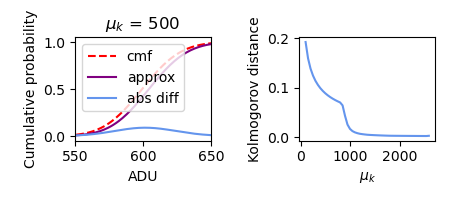
\includegraphics[height=1.0 in]{\images/Kolmogorov}
\includegraphics[height=1.0 in]{\images/Hinton}
\begin{minipage}[b]{7in}
Andrey Kolmogorov, Geoff Hinton: Universal learning algorithms exist. This position is supported by the ``free lunch theorem''.
\end{minipage}

\slide{The No Free Lunch Theorem}

\includegraphics[width=1.0 in]{\images/Chomsky} 

Without prior knowledge, such as universal grammar, it is impossible to make a prediction for an input you have not seen in the training data.


\vfill
{\bf Proof:} Select a predictor $h$ uniformly at random from all functions from ${\cal X}$ to ${\cal Y}$ and then take the data distribution to draw pairs $(x, h(x))$
where $x$ is drawn uniformly from ${\cal X}$.  No learning algorithm can predict $h(x)$ where $x$ does not occur in the training data.


\slide{The Free Lunch Theorem}

Consider a classifier $f$ written in C++ with an arbitrarily large standard library.

\vfill
Let $|f|$ be the number of bits needed to represent $f$.

\vfill
Let $\hat{E}(f) \in [0,1]$ be the error rate on an IID training set and let $E(f)$ be the population error rate.

\vfill
Theorem: With probability at least $1-\delta$ over the draw of the training data the following holds simultaneously for all $f$.

{\color{red} $$E(f) \leq \frac{10}{9}\left(\hat{E}(f) + \frac{5}{N}\left((\ln 2)|f| +\ln\frac{1}{\delta}\right)\right)$$}

\slide{Training Data, Validation Data and Test Data}

Good performance on training data does not guarantee good performance on test data.

\vfill
An nth order polynomial can fit any n (pure noise) data points.

\slide{Loss Vs. Error Rate (or BLEU Score)}
While SGD is generally done on cross entropy loss, one often wants minimum classification error or BLEU Score (for translation).

\vfill
The term ``loss'' often refers to cross entropy loss as opposed to error rate.

\vfill
SGD optimizes loss because error is not differentiable.

\vfill
Later we will discuss attempts to directly optimize error.

\vfill
But training on loss is generally effective.


\slide{Early Stopping}

\centerline{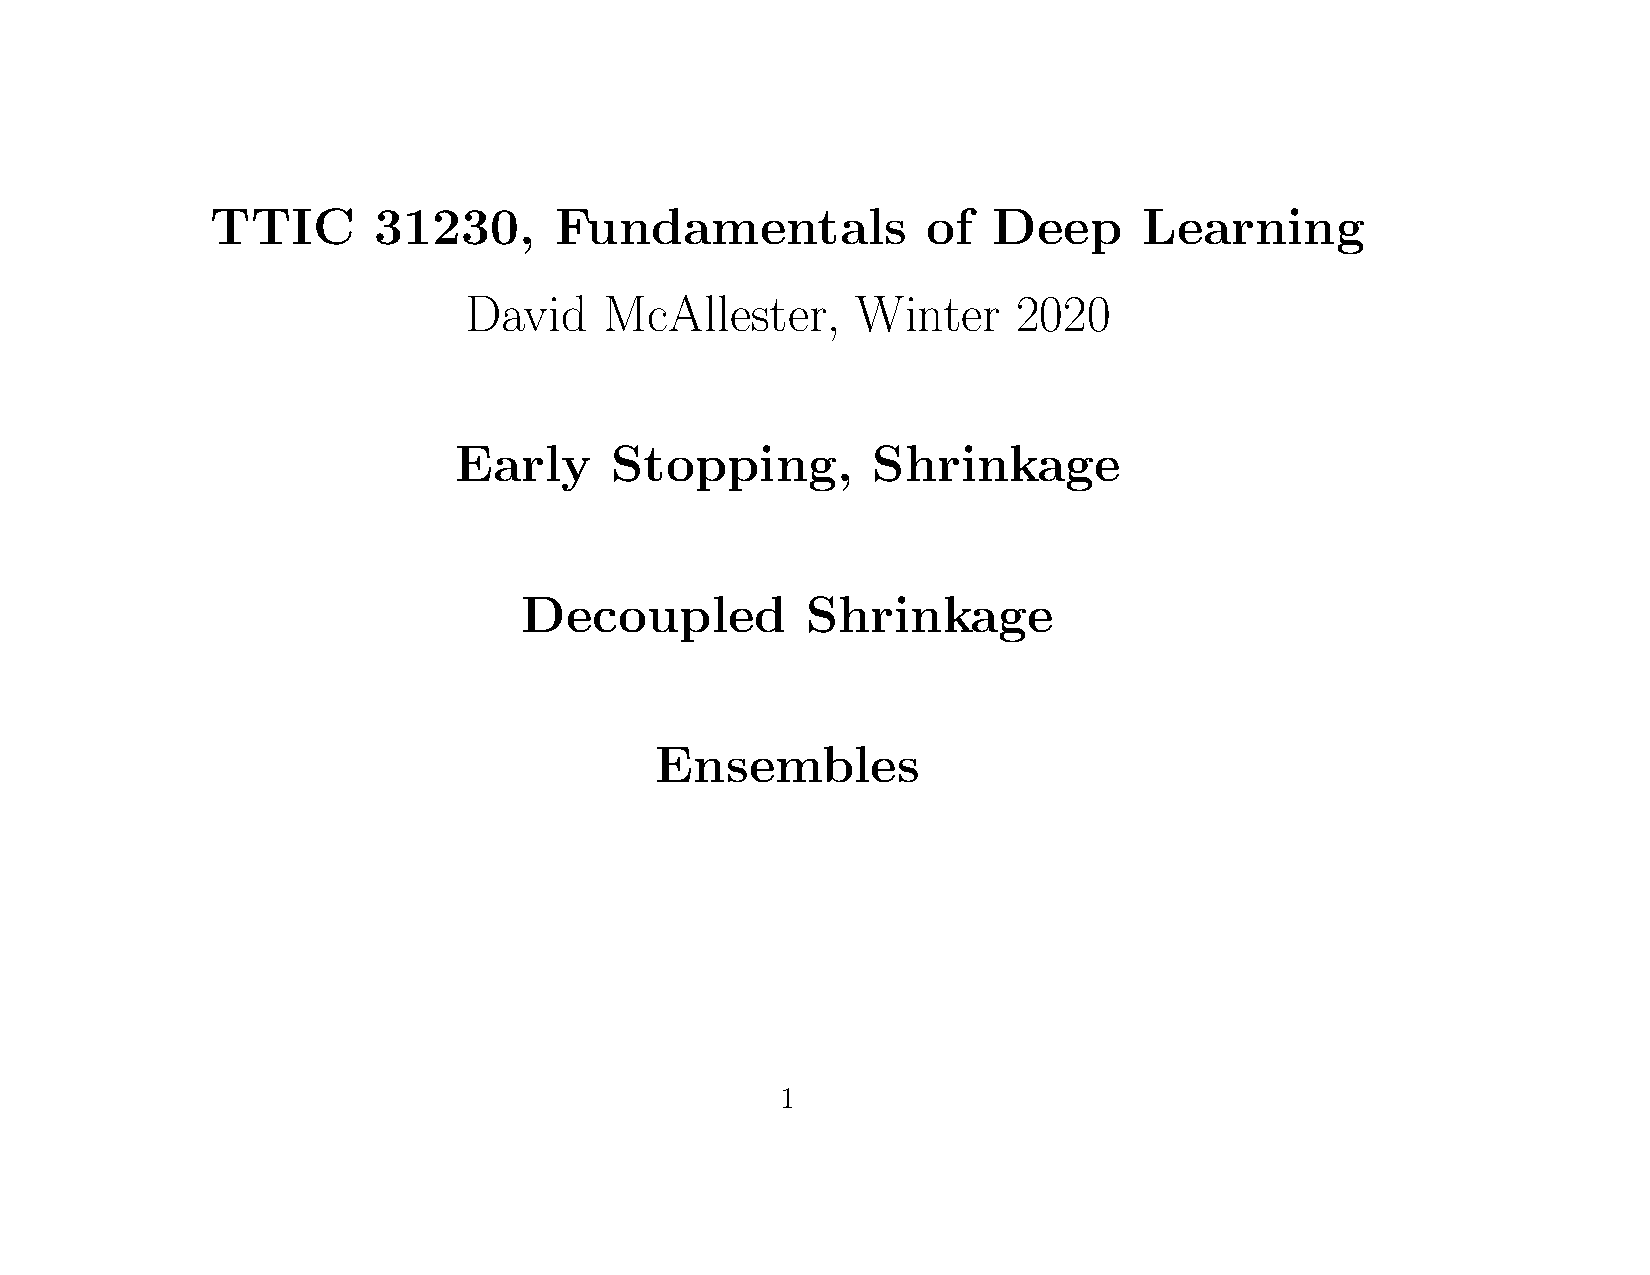
\includegraphics[height = 1.5in]{\images/Early}}

\centerline{\huge Claudia Perlich}

\vfill
During SGD one tracks validation loss or validation error.

\vfill
One stops training when the validation error stops improving.

\vfill
Empirically, loss reaches a minimum sooner than error.

\slide{Training Data, Validation Data and Test Data}

In general one designs algorithms and tunes hyper-parameters by training on training data and evaluating on validation data.

\vfill
But it is possible to over-fit the validation data (validation loss becomes smaller than test loss).

\vfill
Kaggle withholds test data until the final contest evaluation.


\slide{Over Confidence}

\centerline{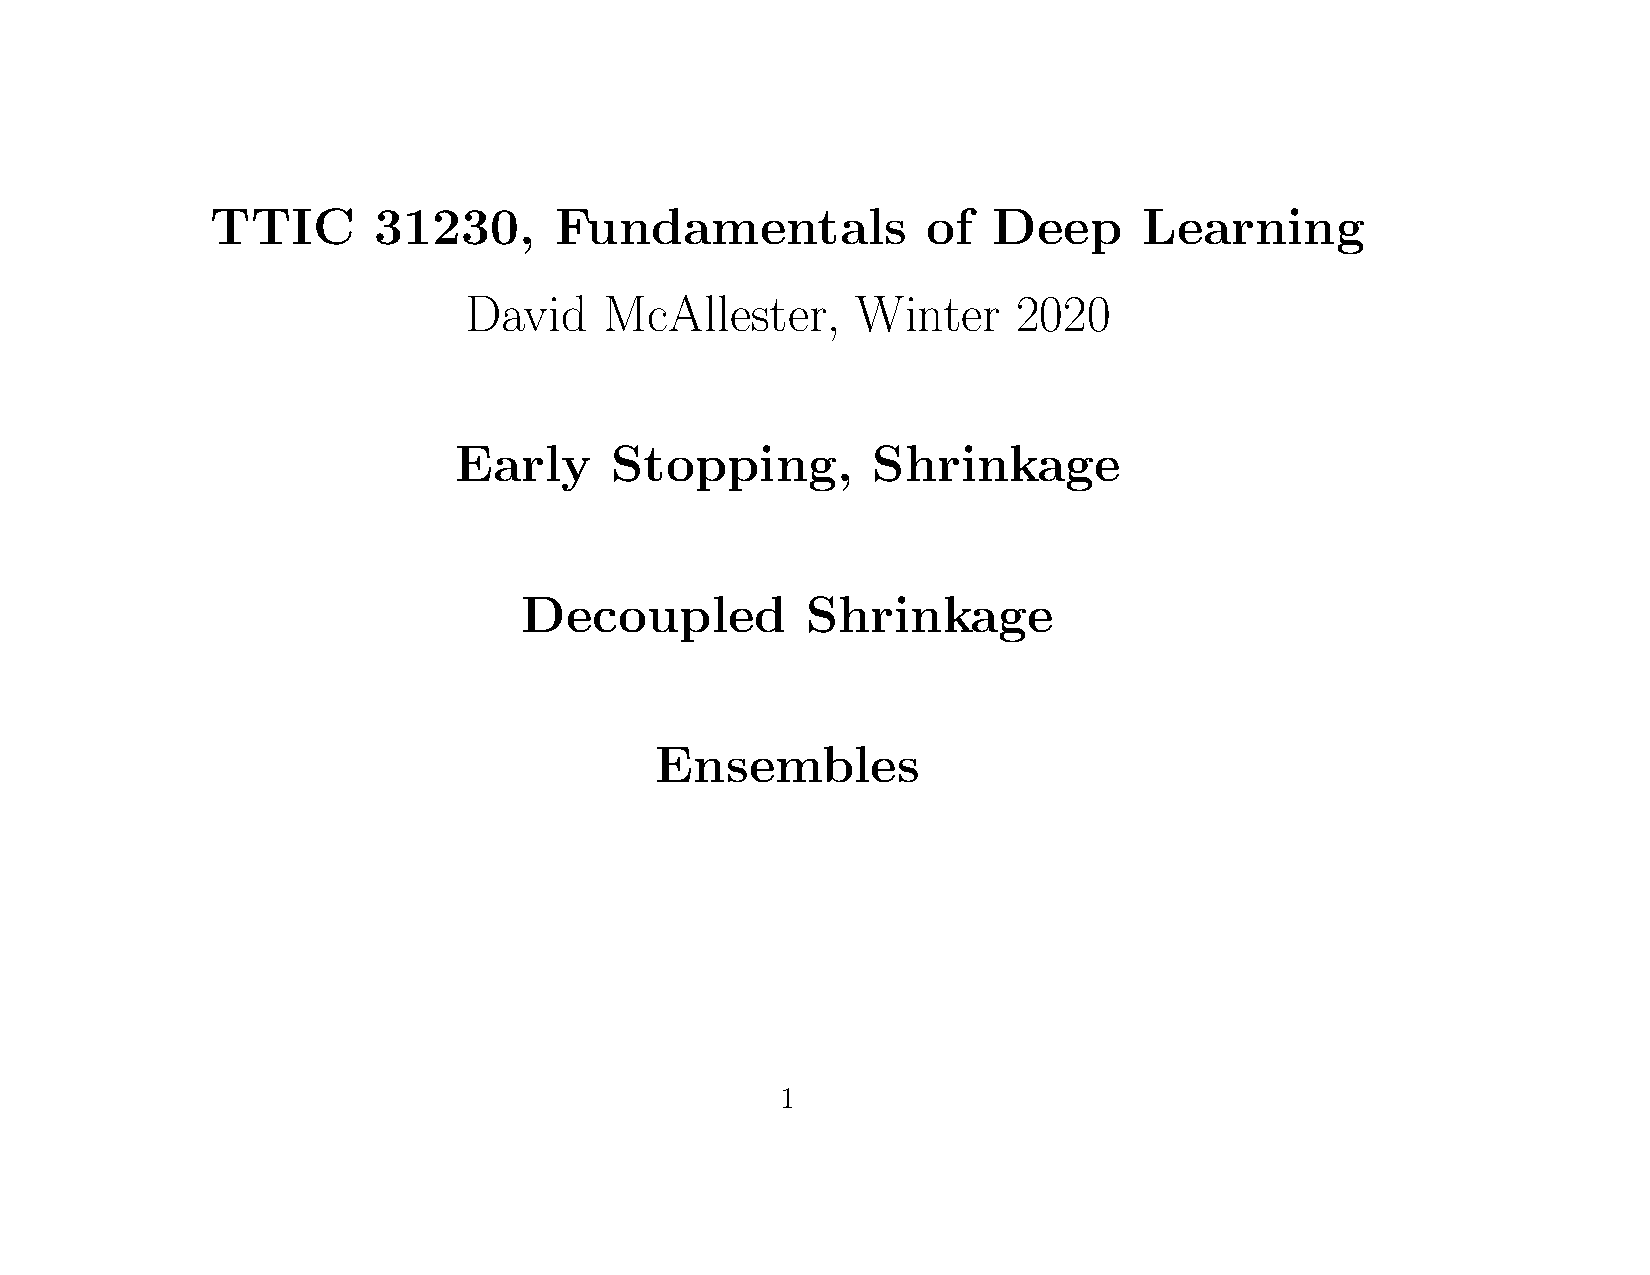
\includegraphics[height = 2in]{\images/Early}}

\vfill
Validation error is larger than training error when we stop.

\vfill
The model probabilities are tuned on training data statistics.

\vfill
The probabilities are tuned to an unrealistically low lower error rate and are therefore over-confident.

\vfill
This over-confidence occurs before the stopping point and damages validation loss.

\slide{Regularization}

There is never harm in doing early stopping --- one should always do early stopping.

\vfill
Regularization is a modification to the training algorithm designed to reduce the training-validation gap and, in this way, improving overall performance.

\slide{$L_2$ Regularization}

Will first give a Bayesian derivation. We put a prior probability on $\Phi$ and maximize the posteriori probability (MAP).

\vfill
\begin{eqnarray*}
\Phi^* & = & \argmax_\Phi\;p(\Phi | \tuple{x_1,y_1},\ldots,\tuple{x_n,y_n}) \\
\\
 & = & \argmax_\Phi\;p(\Phi,\;\tuple{x_1,y_1},\ldots,\tuple{x_n,y_n}) \\
 \\
 & = & \argmax_\Phi \; p(\Phi)\;\prod_i P_\Phi(y_i|x_i) \\
 \\
 & = & \argmin_\Phi -\ln  p(\Phi) + \sum_i - \ln P_\Phi(y_i|x_i)
 \end{eqnarray*}

\slide{$L_2$ Regularization}

Take a Gaussian prior {\color{red} $$p(\Phi) \propto \exp\left(-\frac{||\Phi||^2}{2\sigma^2}\right)$$}

\vfill
\begin{eqnarray*}
\Phi^* & = & \argmin_\Phi \sum_i - \ln P_\Phi(y_i|x_i) -\ln  p(\Phi)  \\
\\
& = & \argmin_\Phi \sum_{i = 1}^n - \ln P_\Phi(y_i|x_i) + \frac{||\Phi||^2}{2\sigma^2}  \\
\\
& = & \argmin_\Phi E_{\tuple{x,y}\sim \mathrm{Train}}\;-\ln P(y|x) + \frac{1}{2N\sigma^2} ||\Phi||^2
\end{eqnarray*}

\slide{Applying SGD}

\begin{eqnarray*}
  & & \nabla_\Phi \;E_{(x,y) \sim \mathrm{Train}}\;\left({\cal L}(\Phi,x,y) + \frac{||\Phi||^2}{2N\sigma^2}\right) \\
  \\
  \\
  & = & E_{(x,y) \sim \mathrm{Train}} \;\left(g(\Phi,x,y) + \frac{\Phi}{N\sigma^2}\right)
\end{eqnarray*}

\vfill
{\color{red} $$\Phi \;\minuseq\; \eta\hat{g} +\frac{\eta}{N\sigma^2}\Phi$$}

\slide{Decoupling Hyperparameters}

$${\color{red} \Phi_{t+1}} = \Phi_t - \eta\hat{g} - \frac{\eta}{N\sigma^2}\Phi_t\;\;\;\; = {\color{red} \Phi_t - \eta\hat{g} - \gamma\Phi_t}$$

\vfill
We can the PyTorch shinkage parameter $\gamma$ to be 
\vfill
{\color{red} $$\gamma = \frac{\eta}{N_{\mathrm{Train}}\sigma^2} = \frac{B\eta_0}{N_gN_{\mathrm{Train}}\sigma^2}$$}

\vfill
The decoupled shrinkage parameter $\sigma$ should then be decoupled from the bath size $B$, the decoupled learning rate $\eta_0$, the momentum parameter $N_g$ and
the size of the training corpus $N_{\mathrm{Train}}$.

\slide{Shrinkage meets Early Stopping}

Early stopping can limit $||\Phi||$.

\vfill
But early stopping more directly limits $||\Phi - \Phi_\mathrm{init}||$.

\vfill
It seems better to take the prior on $\Phi$ to be

\vfill
{\color{red} $$p(\Phi) \propto \exp\left(-\frac{||\Phi - \Phi_{\mathrm{init}}||^2}{2\sigma^2}\right)$$}

\vfill
giving

\vfill
$$\Phi_{t+1} = \Phi_t - \eta\hat{g} - \gamma(\Phi_t - \Phi_{\mathrm{init}})$$

\slide{A Generalization Guarantee}

Assume $0 \leq {\cal L}(\Phi,x,y) \leq \lmax$.

\vfill
Define:
\begin{eqnarray*}
{\cal L}(\Phi) & = & E_{\;(x,y)\sim \pop,\;\epsilon \sim {\cal N}(0,\sigma)^d}\;{{\cal L}(\Phi+\epsilon,x,y)} \\
\\
\hat{{\cal L}}(\Phi) & = & E_{\;(x,y)\sim \mathrm{Train},\;\epsilon \sim {\cal N}(0,\sigma)^d}\;{{\cal L}(\Phi+\epsilon,x,y)} \\
\end{eqnarray*}

\vfill
Theorem: With probability at least $1-\delta$ over the draw of training data the following holds {\bf simultaneously} for all $\Phi$.
\begin{eqnarray*}
   {\color{red} {\cal L}(\Phi)} & {\color{red} \leq} & {\color{red} \frac{10}{9}\parens{\hat{{\cal L}}(\Phi)
   + \frac{5 \lmax}{N_{\mathrm{train}}}\parens{\frac{||\Phi-\Phi_{\mathrm{init}}||^2}{2\sigma^2} + \ln \frac{1}{\delta}}}}
\end{eqnarray*}


\slide{PAC-Bayesian Guarantees}

\vfill
In the PAC-Bayesian framework we assume a prior distribution (or density) on models.

\vfill
For any prior (true or not) selected before seeing the data, any model with sufficiently large prior probability is guaranteed to have the generalization loss near the training loss.

\vfill
For the shrinkage bound the prior is $p(\Phi) \propto  \exp\left(\frac{-||\Phi -\Phi_{\mathrm{init}}||^2}{2\sigma^2}\right)$.

\begin{eqnarray*}
   {\color{red} {\cal L}(\Phi)} & {\color{red} \leq} & {\color{red} \frac{10}{9}\parens{\hat{{\cal L}}(\Phi)
   + \frac{5 \lmax}{N}\parens{\frac{||\Phi-\Phi_{\mathrm{init}}||^2}{2\sigma^2} + \ln \frac{1}{\delta}}}}
\end{eqnarray*}


\slide{A Simpler Theorem}

Consider any prior probability $P(h)$ over an discrete class ${\cal H}$.

\vfill
Assume $0 \leq {\cal L}(h,x,y) \leq \lmax$.

\vfill
Define:
\begin{eqnarray*}
{\cal L}(h)  & = &  E_{(x,y)\sim \mathrm{Pop}}\;{\cal L}(h,x,y) \\
\\
\hat{{\cal L}}(h) & = & E_{(x,y)\sim \mathrm{Train}}\;{\cal L}(h,x,y)
\end{eqnarray*}

\vfill
    {\bf Theorem:} With probability
    at least $1-\delta$ over the draw of training data the following holds simultaneously for all $h$.

\vfill
    $${\cal L}(h) \leq \frac{10}{9}\parens{\hat{\cal L}(h) + \frac{5 L_\mathrm{max}}{N}\parens{\ln \frac{1}{P(h)} + \ln\frac{1}{\delta}}}$$

\slide{Proof}

Consider $\lmax = 1$ and define $\epsilon(h)$ by

\vfill
$$\epsilon(h) = \sqrt{\frac{2{\cal L}(h)\parens{\ln\frac{1}{P(h)} + \ln\frac{1}{\delta}}}{N}}.$$

\vfill
By the relative Chernov bound we have

\vfill
$$P_{\mathrm{Train} \sim \mathrm{Pop}}\parens{\hat{{\cal L}}(h) \leq {\cal L}(h) - \epsilon(h)} \leq e^{-N\frac{\epsilon(h)^2}{2{\cal L}(h)}} = \delta P(h).$$

\slide{Proof}

$$P_{\mathrm{Train} \sim \mathrm{Pop}}\parens{\hat{{\cal L}}(h) \leq {\cal L}(h) - \epsilon(h)} \leq \delta P(h).$$

\vfill
$$P_{\mathrm{Train} \sim \mathrm{Pop}}\parens{\exists h\;\hat{{\cal L}}(h) \leq {\cal L}(h) - \epsilon(h)} \leq \sum_h \delta P(h) =\delta$$

\vfill
$$P_{\mathrm{Train} \sim \mathrm{Pop}}\parens{\forall h\;{\cal L}(h) \leq \hat{{\cal L}}(h) + \epsilon(h)} \geq 1- \delta$$

\slide{Proof}

$${\cal L}(h) \leq \widehat{{\cal L}}(h) + \sqrt{{\cal L}(h)\parens{\frac{2\parens{\ln\frac{1}{P(h)} + \ln\frac{1}{\delta}}}{N}}}$$

using
$$\sqrt{ab} = \inf_{\lambda > 0}\;\frac{a}{2\lambda} + \frac{\lambda b}{2}$$
\vfill
we get
$${\cal L}(h) \leq \widehat{{\cal L}}(h) + \frac{{\cal L}(h)}{2\lambda} + \frac{\lambda\parens{\ln\frac{1}{P(h)} + \ln\frac{1}{\delta}}}{N}$$

\slide{Proof}
$${\cal L}(h) \leq \widehat{{\cal L}}(h) + \frac{{\cal L}(h)}{2\lambda} + \frac{\lambda\parens{\ln\frac{1}{P(h)} + \ln\frac{1}{\delta}}}{N}$$

\vfill
Solving for ${\cal L}(h)$ yields

\vfill
$${\cal L}(h) \leq \frac{1}{1-\frac{1}{2\lambda}}\parens{\hat{{\cal L}}(h) + \frac{\lambda}{N}\parens{\ln \frac{1}{P(h)} + \ln \frac{1}{\delta}}}$$

\vfill
Setting $\lambda = 5$ and rescaling the loss gives the version on earlier slides.

\slide{A Model Compression Guarantee}

Let $|\Phi|$ be the number of bits used to represent $\Phi$ under some fixed compression scheme.

\vfill
Let $P(\Phi) = 2^{-|\Phi|}$

\vfill
    $${\cal L}(\Phi) \leq \frac{10}{9}\parens{\hat{\cal L}(\Phi) + \frac{5 L_\mathrm{max}}{N}\parens{(\ln 2)|\Phi| + \ln\frac{1}{\delta}}}$$

\slide{Adding Noise Simulates Limiting Precision}

Assume $0 \leq {\cal L}(\Phi,x,y) \leq \lmax$.

\vfill
Define:
\begin{eqnarray*}
{\cal L}(\Phi) & = & E_{\;(x,y)\sim \pop,\;\epsilon \sim {\cal N}(0,\sigma)^d}\;{{\cal L}(\Phi+\epsilon,x,y)} \\
\\
\hat{{\cal L}}(\Phi) & = & E_{\;(x,y)\sim \mathrm{Train},\;\epsilon \sim {\cal N}(0,\sigma)^d}\;{{\cal L}(\Phi+\epsilon,x,y)} \\
\end{eqnarray*}

\vfill
Theorem: With probability at least $1-\delta$ over the draw of training data the following holds {\bf simultaneously} for all $\Phi$.
\begin{eqnarray*}
   {\color{red} {\cal L}(\Phi)} & {\color{red} \leq} & {\color{red} \frac{10}{9}\parens{\hat{{\cal L}}(\Phi)
   + \frac{5 \lmax}{N}\parens{\frac{||\Phi-\Phi_{\mathrm{init}}||^2}{2\sigma^2} + \ln \frac{1}{\delta}}}}
\end{eqnarray*}

\slide{A KL Divergence Bound}

Let $P$ be any ``prior'' and $Q$ be any ``posterior'' on any model space.

\vfill
Define
\begin{eqnarray*}
  L(Q) & =  &\expectsub{h \sim Q}{L(h)} \\
  \\
  \hat{L}(Q) & =  &\expectsub{h \sim Q}{\hat{L}(h)}
\end{eqnarray*}


\vfill
For any $P$ and any $\lambda > \frac{1}{2}$, with probability
at least $1-\delta$ over the draw of the training data, the following holds simultaneously for all $Q$.
\vfill
$$L(Q) \leq \frac{1}{1-\frac{1}{2\lambda}}\parens{\hat{L}(Q) + \frac{\lambda \lmax}{N}\parens{KL(Q,P) + \ln \frac{1}{\delta}}}$$


\slide{$L_1$ Regularization and Sparse Weights}

$$p(\Phi) \propto e^{-\lambda ||\Phi||_1} \;\;\;\;\;\;\;\;||\Phi||_1 = \sum_i |\Phi_i|$$

$$\Phi^* = \argmin_\Phi \; \;\;\hat{\cal L}(\Phi) \;+ \; \;\frac{\lambda}{N_{\mathrm{train}}}||\Phi||_1$$

\begin{eqnarray*}
  \Phi & \minuseq & \eta \nabla_\Phi \; \hat{\cal L}(\Phi) \\
  \Phi_i & \minuseq & (\eta\lambda/N_{\mathrm{train}})\; \mathrm{sign}(\Phi_i) \;\;\;\;\;\;\mbox{(shrinkage)}
\end{eqnarray*}

\vfill
At equilibrium \hfill (sparsity is difficult to achieve with SGD)

$$\begin{array}{rcll}
\Phi_i &  = & 0  & \;\;\;\;\;\mbox{if} \;\left|\partial {\cal L} /\partial \Phi_i\right| <  \lambda/N_{\mathrm{train}} \\
\partial {\cal L} /\partial \Phi_i & = &  -(\lambda/N_{\mathrm{train}}) \mathrm{sign}(\Phi_i) &\;\;\;\;\; \mbox{otherwise}
\end{array}$$


\slide{Ensembles}

Train several models $\mathrm{Ens} = (\Phi_1,\;\ldots,\; \Phi_k)$ from different initializations and/or under different meta parameters.

\vfill
We define the ensemble model by
$$P_\mathrm{Ens}(y|x) = \frac{1}{k} \sum_{j=1}^k\; P_{\Phi_i}(y|x)$$

\vfill
Ensemble models almost always perform better than any single model.


\vfill
\slide{Ensembles Under Cross Entropy Loss}

For log loss we average the probabilities.

\vfill
$$P(y|x) = \frac{1}{k} \sum_i \;P_i(y|x)$$

\vfill
$- \log P$ is a convex function of $P$.  For any convex ${\cal L}(P)$ Jensen's inequality states that

$${\cal L}\left(\frac{1}{k} \sum_i P_i\right) \leq \frac{1}{k} \sum_i {\cal L}(P_i)$$

\vfill
This implies that the loss of the average model cannot be worse (can only be better) than the average loss of the models.

\vfill
\slide{Ensembles Under Cross Entropy Loss}

By Jensen:

$${\cal L}\left(\frac{1}{k} \sum_i P_i\right) \leq \frac{1}{k} \sum_i {\cal L}(P_i)$$

\vfill
However, in practice for each $i$ we have

$${\cal L}\left(\frac{1}{k} \sum_i P_i\right) \leq {\cal L}(P_i)$$

\ignore{
\slide{Ensembles under Square Loss}

We average $k$ regression models

\vfill
\begin{eqnarray*}
  f(x) & = & \frac{1}{k} \sum_{i=1}^k\; f_i(x) \\
  \\
  \\
  f(x) - y & = & \frac{1}{k} \sum_{i=1}^k\; (f_i(x) - y) \\
  \\
  \\
  \epsilon & = & \frac{1}{k}  \sum_{i=1}^k\; \epsilon_i,\;\;\epsilon_i = f_i - y \;\;\;\mbox{(residuals)}
\end{eqnarray*}



\slide{Ensembles for Square Loss}

Assume that $\expect{\epsilon_i ^2} = \sigma^2$ and $\expect{\epsilon_i \epsilon_j} = \sigma^2\rho$ for $i \not = j$.

\begin{eqnarray*}
  \expect{\left(\frac{1}{k} \sum_i \epsilon_i\right)^2} & = & \frac{1}{k^2} \expect{\sum_i\;\left(\epsilon_i^2 + \sum_{j \not = i}\;\epsilon_i\epsilon_j\right)} \\
  \\
  \\
  & = & \frac{1}{k} \sigma^2 + \frac{k-1}{k} \sigma^2\rho \;=\; \sigma^2\left(\frac{1}{k} + \left(1-\frac{1}{k}\right)\rho\right)
\end{eqnarray*}

\vfill
If Pearson's correlation $\rho = \expect{\epsilon_i\epsilon_j}/\sigma^2 < 1$ we win.
}


\slide{Implicit Regularization}

Any stochastic learning algorithm, such as SGD, determines a stochastic mapping from training data to models.

\vfill
The algorithm can implicitly incorporate a preference or bias for models.

\vfill
For example, solving linear regression with many more parameters than data points
has many solutions.

\vfill
But SGD finds converges to the minimum norm solution.

\slide{Implicit Regularization}

SGD maintains the invariant that $\Phi$ is a linear combination of the (small number of) training vectors.

\vfill
Any zero-loss (squared loss) solution can be projected on the span of training vectors to give a no larger norm solution.

\vfill
It can be shown that any zero loss solution in the span of the training vectors is a least-norm solution.

\slideplain{An Implicit Regularization Generalization Guarantee}

Let ${\cal H}$ be a discrete set of classifiers.

\vfill
Let $A$ be an algorithm mapping a training set to a classifier.

\vfill
Let $P(h | A,\pop)$ be the probability over the draw of the training data that $A(\mathrm{Train}) = h$.

\vfill
Theorem: With probability at least $1-\delta$ over the draw of the training data we have
$${\color{red} \mathrm{Err}(A(\mathrm{Train}))} \leq \frac{10}{9}\parens{\begin{array}{l} {\color{red} \hat{\mathrm{Err}}(A(\mathrm{Train}))}
 \\+ \frac{5}{N}\parens{
\ln \frac{1}{{\color{red} P(A(\mathrm{Train})|A,\pop)}} + \ln \frac{1}{\delta}}\end{array}}$$


\ignore{
\slide{Optimality of $Q_{\cal A}(\mathrm{Pop})$}

Consider an arbitrary prior $P$.

\vfill
\begin{eqnarray*}
  & & E_{\mathrm{Train}\sim\mathrm{Pop}}\;KL(Q_{\cal A}(\mathrm{Train}),P) \\
  \\
  & = & E_{\mathrm{Train}\sim\mathrm{Pop}}\;\ln \frac{Q_{\cal A}(\mathrm{Train})(h)}{P(h)}  \\
\\
\\
& = & \expectsub{\mathrm{Train}\sim \mathrm{Pop},\;h \sim Q_{\cal A}(\mathrm{Train})}{\ln \frac{Q_{\cal A}(\mathrm{Train})(h)}{Q_{\cal A}(\mathrm{Pop})(h)}} \\
\\
\\
& & + \expectsub{h \sim Q_{\cal A}(\mathrm{Pop})}{\ln \frac{Q_{\cal A}(\mathrm{Pop}(h))}{P(h)}}
\end{eqnarray*}

\slideplain{Optimality of $Q_{\cal A}(\mathrm{Pop})$}

\begin{eqnarray*}
  & & E_{\mathrm{Train}\sim\mathrm{Pop}}\;KL(Q_{\cal A}(\mathrm{Train}),P) \\
\\
& = & \expectsub{\mathrm{Train}\sim \mathrm{Pop}}{KL(Q_{\cal A}(\mathrm{Train}),Q_{\cal A}(\mathrm{Pop}))} + KL(Q_{\cal A}(\mathrm{Pop}),P)
\end{eqnarray*}

\vfill
So $Q_{\cal A}(\mathrm{Pop})$ is an {\bf optimal prior} (or {\bf implicit prior}) for algorithm ${\cal A}$.
}

\ignore{
\slide{The Broad Basin Hypothesis}

Do broad basins in the loss function generalize better?

\vfill

{\bf Flat Minima:} Hochreiter and Schmidhuber (1997)

\vfill
{\bf On Large-Batch Training for Deep Learning: Generalization Gap and Sharp Minima:} Keskar et al. (Nocedal) arXiv 2016, ICLR 2017.

\vfill
{\bf Sharp Minima Can Generalize For Deep Nets:} Dihn et al. (both Bengios) arXiv 2017.

\vfill
I believe that the PAC-Bayesian analysis supports the broad basin hypothesis.  We are interested in the implicit prior (implicit geometry) of SGD
and ``broad'' should be defined in terms of that geometry.
}

\ignore{
\slide{Sparse Activation}

We can impose an $L_1$ regularization on the activations of the network (the output of the activation function of each neuron).

$$\Phi^* = \argmin_\Phi {\cal L}(\Phi) + \lambda||h||_1$$

\vfill
where $h$ is the vector of neuron activation outputs.

\vfill
This will tend to make activations sparse.

\slide{Sparse Coding}

Let $W$ be a matrix where we view $W_{\cdot,i}$ is the $i$th ``dictionary vector''.

\vfill
For input $x$ we can construct a $k$-sparse representation $h(x)$.

\vfill
$$h(x) = \argmin_{h,||h||_0=k} \;||x - Wh||^2$$

\vfill
Note

$$Wh = \sum_{i \in I(x)} \; h_i \; W_{\cdot,i}\;\;\;\;\;|I(x)| = k$$

\vfill
We can now replace $x$ by its sparse code $h(x)$.

}

\ignore{
\slide{Modeling the Implicit Prior}

We divide the parameters into classes where we write $c_i$ for the class of parameter $w_i$.

\vfill
We let $w_i^0$ be the initial value of $w_i$ and let $w_i^f(S)$ be the final value of $w_i$.

\vfill
\begin{eqnarray*}
\beta_{c,1},\beta_{c,2} & = & E_{S \sim D^N}\;\argmin_{\beta_1,\beta_2}\; \sum_{i: c_i = c}\;(w_i^f(S) - (\beta_1 w_i^0 + \beta_2))^2 \\
\beta_{c,3},\beta_{c,4} &  = & E_{S \sim D^N}\; \argmin_{\beta_3,\beta_4}\;\sum_{i: c_i = c}\;((w_i^f(S) - (\beta_{c_1,1} w_i^0 + \beta_{c_i,2}))^2 - (\beta_3 w_i^0 + \beta_4))^2
\end{eqnarray*}

We then consider the prior distribution $P$ on $w_i$ to be a Gaussian with mean $\mu_i$ and standard deviation $\sigma_i$ given by

\begin{eqnarray*}
  \mu_i & = & \beta_{c_i,1}w_i^0 + \beta_{c_i,2} \\
  \sigma_i^2 & = & \beta_{c_i,3}w_i^0 + \beta_{c_i,4}
\end{eqnarray*}

\slide{Modeling the Implicit Prior}

This prior does not depend on any particular training data $S$ and hence is a legitimate prior.

\vfill
In practice we can estimate this prior from the training data.

\begin{eqnarray*}
\hat{\beta}_{c,1},\hat{\beta}_{c,2} & = & \argmin_{\beta_1,\beta_2} \sum_{i: c_i = c}\;(w_i^f(S) - (\beta_1 w_i^0 + \beta_2))^2 \\
\hat{\beta}_{c,3},\hat{\beta}_{c,4} &  = & \argmin_{\beta_3,\beta_4} \sum_{i: c_i = c}\;((w_i^f(S) - (\hat{\beta}_{c_i,1} w_i^0 + \hat{\beta}_{c_i,2}))^2 - (\beta_3 w_i^0 + \beta_4))^2
\end{eqnarray*}
}

\slide{Dropout}

Dropout can be viewed as an ensemble method.


\vfill
To draw a model from the ensemble we randomly select a mask $\mu$ with

$$\left\{\begin{array}{ll} \mu_i = 0 & \mbox{with probability $\alpha$} \\ \\ \mu_i = 1 & \mbox{with probability $1-\alpha$}
\end{array}\right.$$

\vfill
Then we use the model $(\Phi,\;\mu)$ with weight layers defined by


\vfill
$$y_i = \mathrm{Relu}\left(\sum_j\;W_{i,j} \;\mu_jx_j\right)$$

\slide{Dropout Training}

Repeat:

\vfill

\begin{itemize}
\item Select a random dropout mask $\mu$
  
\vfill
\item $\Phi \;\minuseq\; \nabla_\Phi\; {\cal L}(\Phi, \mu)$
\end{itemize}

\vfill
Backpropagation must use the same mask $\mu$ used in the forward computation.

\slide{Test Time Scaling}


\vfill
At train time we have

\vfill
$$y_i = \mathrm{Relu}\left(\sum_j\;W_{i,j} \;\mu_j x_j\right)$$


\vfill
At test time we have

\vfill
$$y_i = \mathrm{Relu}\left((1-\alpha)\;\sum_j\;W_{i,j} \;x_j\right)$$

\vfill
At test time we use the ``average network''.

\slide{Dropout for Least Squares Regression}

Consider simple least square regression

\begin{eqnarray*}
  \Phi^* & = &  \argmin_\Phi\;\; \mathrm{E}_{(x,y)} \;\expectsub{\mu}{(y - \Phi \cdot (\mu \odot x))^2} \\
  \\
  & = & \expect{(\mu\odot x)(\mu\odot x)^{\top}}^{-1}\; \expect{y (\mu\odot x)} \\
  \\
  & = & \argmin_\Phi\;\; \mathrm{E}_{(x,y)} (y - (1-\alpha) \Phi \cdot x)^2 + \sum_i\frac{1}{2}(\alpha - \alpha^2) \expect{x_i^2} \Phi_i^2
\end{eqnarray*}

\vfill
In this case dropout is equivalent to a form of $L_2$ regularization --- see Wager et al. (2013).

\slide{Model Compression}

Deep Compression: Compressing Deep Neural
Networks With Pruning, Trained Quantization
and Huffman Coding, Han et al., ICLR 2016.

\vfill
\begin{itemize}
\item Compressed Models can be downloaded to mobile devices faster and fit in lower-power CPU memory.  (The motivation of this paper).

\vfill
\item Sparse models may be more interpretable than dense models.

\vfill
\item Model size is a measure of model complexity and can be viewed as a form of regularization.
\end{itemize}

\vfill
VGG-16 is reduced by $49 \times$ from 552MB to 11.3MB with no loss of accuracy.

\slide{Three Stages}

\begin{itemize}
\item Sparsification by simple weight thresholding.  ($10 \times$ reduction).

  \vfill
\item Trained Quantization ($6\times$ reduction).

  \vfill
\item Huffman coding ($40\%$ reduction).
\end{itemize}

\slide{Quantization}

They use 5 bits of numerical precision for the weights.

\vfill
This is done by having a table of the 32 possible weight values.

\vfill
We have to cluster the weights into 32 groups and decide on a {\bf centroid value} for each weight.

\vfill
This is done with K-means clustering.

\ignore{
\slide{Initialization of Centroids}

\centerline{\includegraphics[width = 7in]{\images/Compression1}}

\slide{After Running K-means}

\centerline{\includegraphics[width = 7in]{\images/Compression2}}
}

\slide{Retrain to Adjust Centroids}

Run over the data again doing backpropagation to adjust the table of the 32 possible weights.

\vfill
This leaves the 5-bit code of each weight in the model unchanged.

\slide{Huffman Coding}

Different 5-bit numerical codes have different frequencies.

\vfill
This can be viewed as distribution over the 32 code words.

\vfill
We can reduce the average number of bits per weight using fewer bits to code the more common weight values.

\vfill
Huffman coding is applied to both the 5 bit weight coding and a three bit code used in the sparse representation of the weight matrices.

\vfill
This results in about 5 bits  per {\bf nonzero} weight in a {\bf sparse} coding of the weight matrices.

\slide{Dense-Sparse-Dense}

DSD: Dense-Sparse-Dense Training for Deep
Neural Networks, Han et al., ICLR 2017

\vfill
\begin{enumerate}
\item Train a model.

  \vfill
\item Make the model sparse by weight thresholding.

  \vfill
\item Retrain the model holding the sparsity pattern fixed (still 32 bits per weight).

  \vfill
\item Go back to a dense model with all pruned weights initialized to zero.

  \vfill
\item  Retrain the dense model.
\end{enumerate}

Results in significant performance improvements in a wide variety of models.

\slide{Step 1}

\vfill
\centerline{\includegraphics[width = 4in]{\images/DSD1}}

\slide{Step 2}

\vfill
\centerline{\includegraphics[width = 4in]{\images/DSD2}}

\slide{Step 3}

\vfill
\centerline{\includegraphics[width = 4in]{\images/DSD3}}

\slide{Step 4}

\vfill
\centerline{\includegraphics[width = 4in]{\images/DSD4}}

\slide{Step 5}

\vfill
\centerline{\includegraphics[width = 4in]{\images/DSD5}}

\slide{Results}

\vfill
\centerline{\includegraphics[width = 9.5in]{\images/DSDtable}}

\ignore{
\slide{A Dropout Bound}

\begin{eqnarray*}
KL(Q_{\alpha,\Phi},\;Q_{\alpha,0}) & = & \expectsub{\mu \sim P_\alpha, \epsilon \sim {\cal N}(0,1)^d}
{\ln \frac{P_\alpha(\mu) e^{-\frac{1}{2}||\mu \odot \epsilon||^2}}{P_\alpha(\mu) e^{-\frac{1}{2}||\mu \odot (\Phi + \epsilon)||^2}}} \\
\\
& = & \expectsub{\mu \sim P_\alpha}{\frac{1}{2}||\mu \odot \Phi||^2} \\
\\
& = & \frac{1-\alpha}{2}||\Phi||^2
\end{eqnarray*}

$$L(Q_{\alpha,\Phi}) \leq \frac{1}{1-\frac{1}{2\lambda}}\parens{\hat{L}(Q_{\alpha,\Phi}) + \frac{\lambda \lmax}{N}\parens{\frac{1-\alpha}{2}||\Phi||^2 + \ln \frac{1}{\delta}}}$$
}


\slide{Non-Vacuous Generalization Guarantees}

Model compression has recently been used to achieve ``non-vacuous'' PAC-Bayes generalization guarantees for ImageNet classification
--- error rate guarantees less than 1.

\vfill
Non-Vacuous PAC-Bayes Bounds at ImageNet Scale.

\bigskip
Wenda Zhou, Victor Veitch, Morgane Austern, Ryan P. Adams, Peter Orbanz

\bigskip
ICLR 2019

\slide{Double Descent}

{\huge
Reconciling modern machine learning practice and the bias-variance trade-off

\bigskip
Mikhail Belkin, Daniel Hsu, Siyuan Ma, Soumik Mandal, arXiv December 2018.

\vfill
Deep Double Descent: Where Bigger Models and More Data Hurt

\bigskip
Preetum Nakkiran, Gal Kaplun, Yamini Bansal, Tristan Yang, Boaz Barak, Ilya Sutskever, ICLR 2020
}

\slide{Double Descent}

\centerline{\includegraphics[width = 6in]{\images/DoubleDescent1}}

\vfill
Deep Double Descent: Where Bigger Models and More Data Hurt

\bigskip
Preetum Nakkiran, Gal Kaplun, Yamini Bansal, Tristan Yang, Boaz Barak, Ilya Sutskever, ICLR 2020

\slide{Double Descent}

\centerline{\includegraphics[width = 8in]{\images/DoubleDescent2}}

\slide{Summary}

There is never harm in doing early stopping --- one should always do early stopping.

\vfill
Regularization is any modification to the training algorithm motivated by reducing the training-validation gap.

\vfill
While regularization modifications to training can be inspired by theory, the theory is weak.

\vfill
Regularization proposals should be evaluated empirically.

\ignore{
\slide{$L_2$ PAC-Bayesian Bounds in Action}

Computing Nonvacuous Generalization Bounds for Deep (Stochastic) Neural Networks with Many More Parameters than Training Data, (Dziugaite and Roy, arXiv, 2017)

\vfill
\centerline{\includegraphics[width = 8in]{\images/Roy}}

\vfill
{\bf The bounds are based on $L_2$ distance of the weight vector to the initialization.}

\vfill
{\bf The weight vector is retrained to minimize the bound.}
}

\slide{END}

}
\end{document}
